\paragraph{Gestione Questionari}

\label{Recupero dei questionari di un utente}

\begin{figure}[ht]
	\centering
	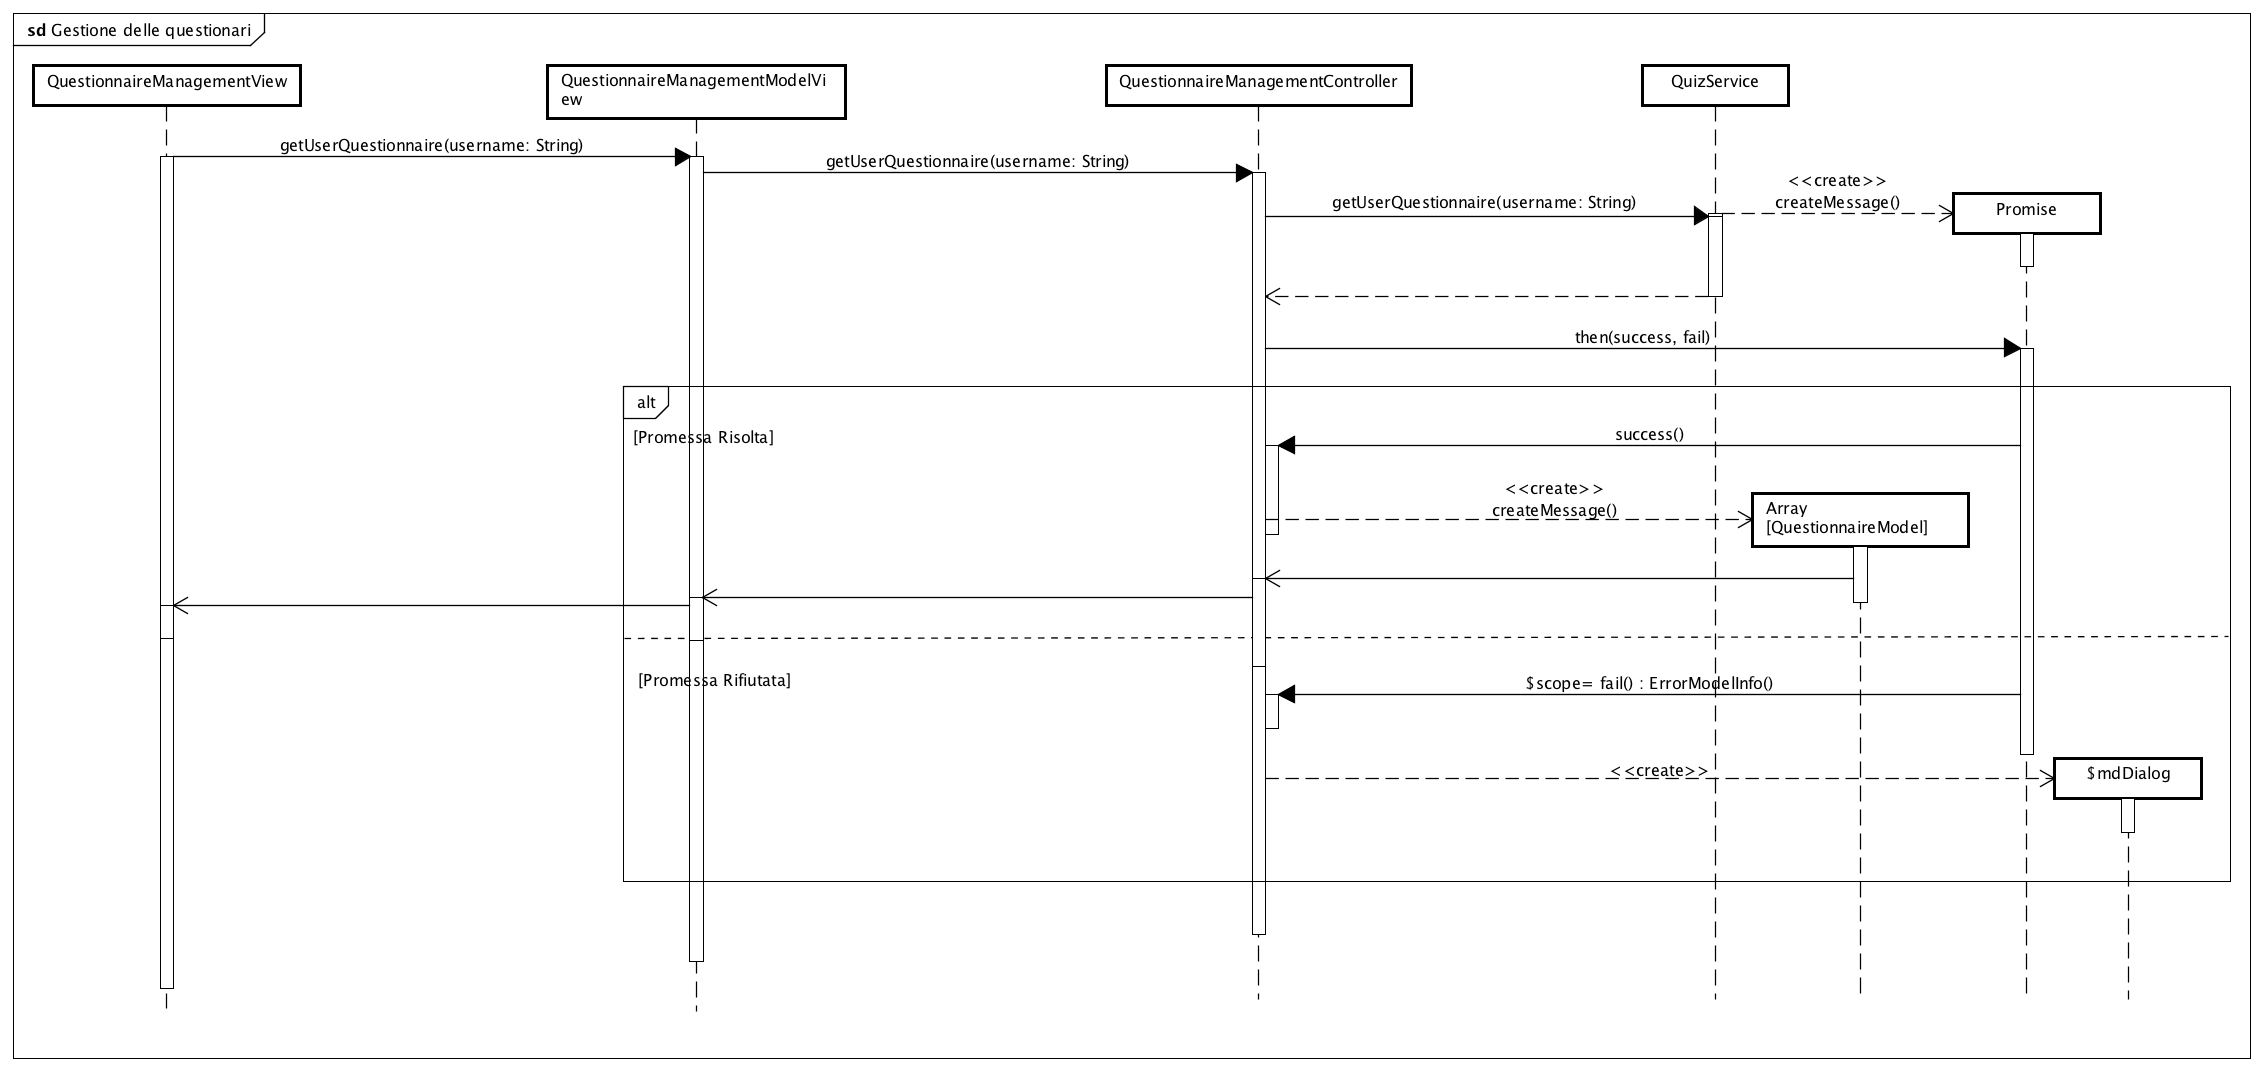
\includegraphics[scale=0.25,keepaspectratio]{UML/DiagrammiDiSequenza/Front-end/QuestionnaireManagement.png}
	\caption{Recupero dei questionari di un utente}
\end{figure} \FloatBarrier

Nella view di visualizzazione domande verrà chiamato il metodo del\\ \texttt{controller\ped{G}} che serve per ottenere tutti questionari create dall'utente autenticato. Il \texttt{controller\ped{G}} eseguirà una richiesta al \texttt{service\ped{G}}. A sua volta il \texttt{service\ped{G}} ritornerà una promessa che potrà essere risolta o rifiutata. Nel caso venga risolta verrà ritornato l'array di tutti i questionari, nel caso invece venga rifiutata verrà restituito un oggetto contenente l'errore e visualizzato un messaggio informativo. 